\section{风险敏感优化}\label{sec:risk}

\begin{chapterquestion}
\textbf{本章研究的问题}：如何避免优化器利用代理模型在低可信区域的盲区？
\end{chapterquestion}

\subsection{风险敏感适应度}

为阻止优化器将粒子推向高 $\sigma$ 的低可信区域，
本文将标准目标 $\mu(x)$ 扩展为风险敏感形式：
\begin{equation}
    \text{Fitness}(x)=\mu(x)-\lambda\,\sigma(x)-P_{\text{scenario}}(x),
    \label{eq:risk}
\end{equation}
其中 $\lambda$ 为风险厌恶系数，$P_{\text{scenario}}$ 为场景软约束惩罚。
当粒子进入训练稀疏/分布外区域时 $\sigma(x)$ 增大，$\lambda\sigma(x)$ 项产生惩罚，
使粒子返回模型置信度较高的区域。
$\lambda=0$ 退化为纯均值最大化（无防护），$\lambda$ 越大越保守。

\textbf{方法定位}：本式与贝叶斯优化中的下置信界（LCB）
$\mu-\beta\sigma$ 共享数学形态，但角色不同：
LCB 是采样策略，本式则直接内嵌于优化目标，
依靠 PSO 群体搜索实现面向可靠性的约束寻优；
其 $\sigma$ 来自集成成员分歧（非高斯过程后验方差）。
因此本方法的定位是\textbf{将不确定性感知思想引入 PSO 框架的一种防御机制}，
而非一种全新的优化范式。它针对的是代理盲区被优化器利用这一可信性问题，
而非寻优速度或最优值的提升。

\subsection{OOD 压力测试}

风险敏感机制的有效性，此前主要来自间接证据
（如 $\lambda=0$ 时适应度越过 100 的反面参照）。
为给出直接证据，本文新增 OOD 压力测试：
系统构造在训练分布内/外的大量输入，比较原始代理 $\mu(x)$
与风险敏感评分 $\mu(x)-\lambda\sigma(x)$ 的行为（$\lambda=1$）。

\begin{figure}[H]
\centering
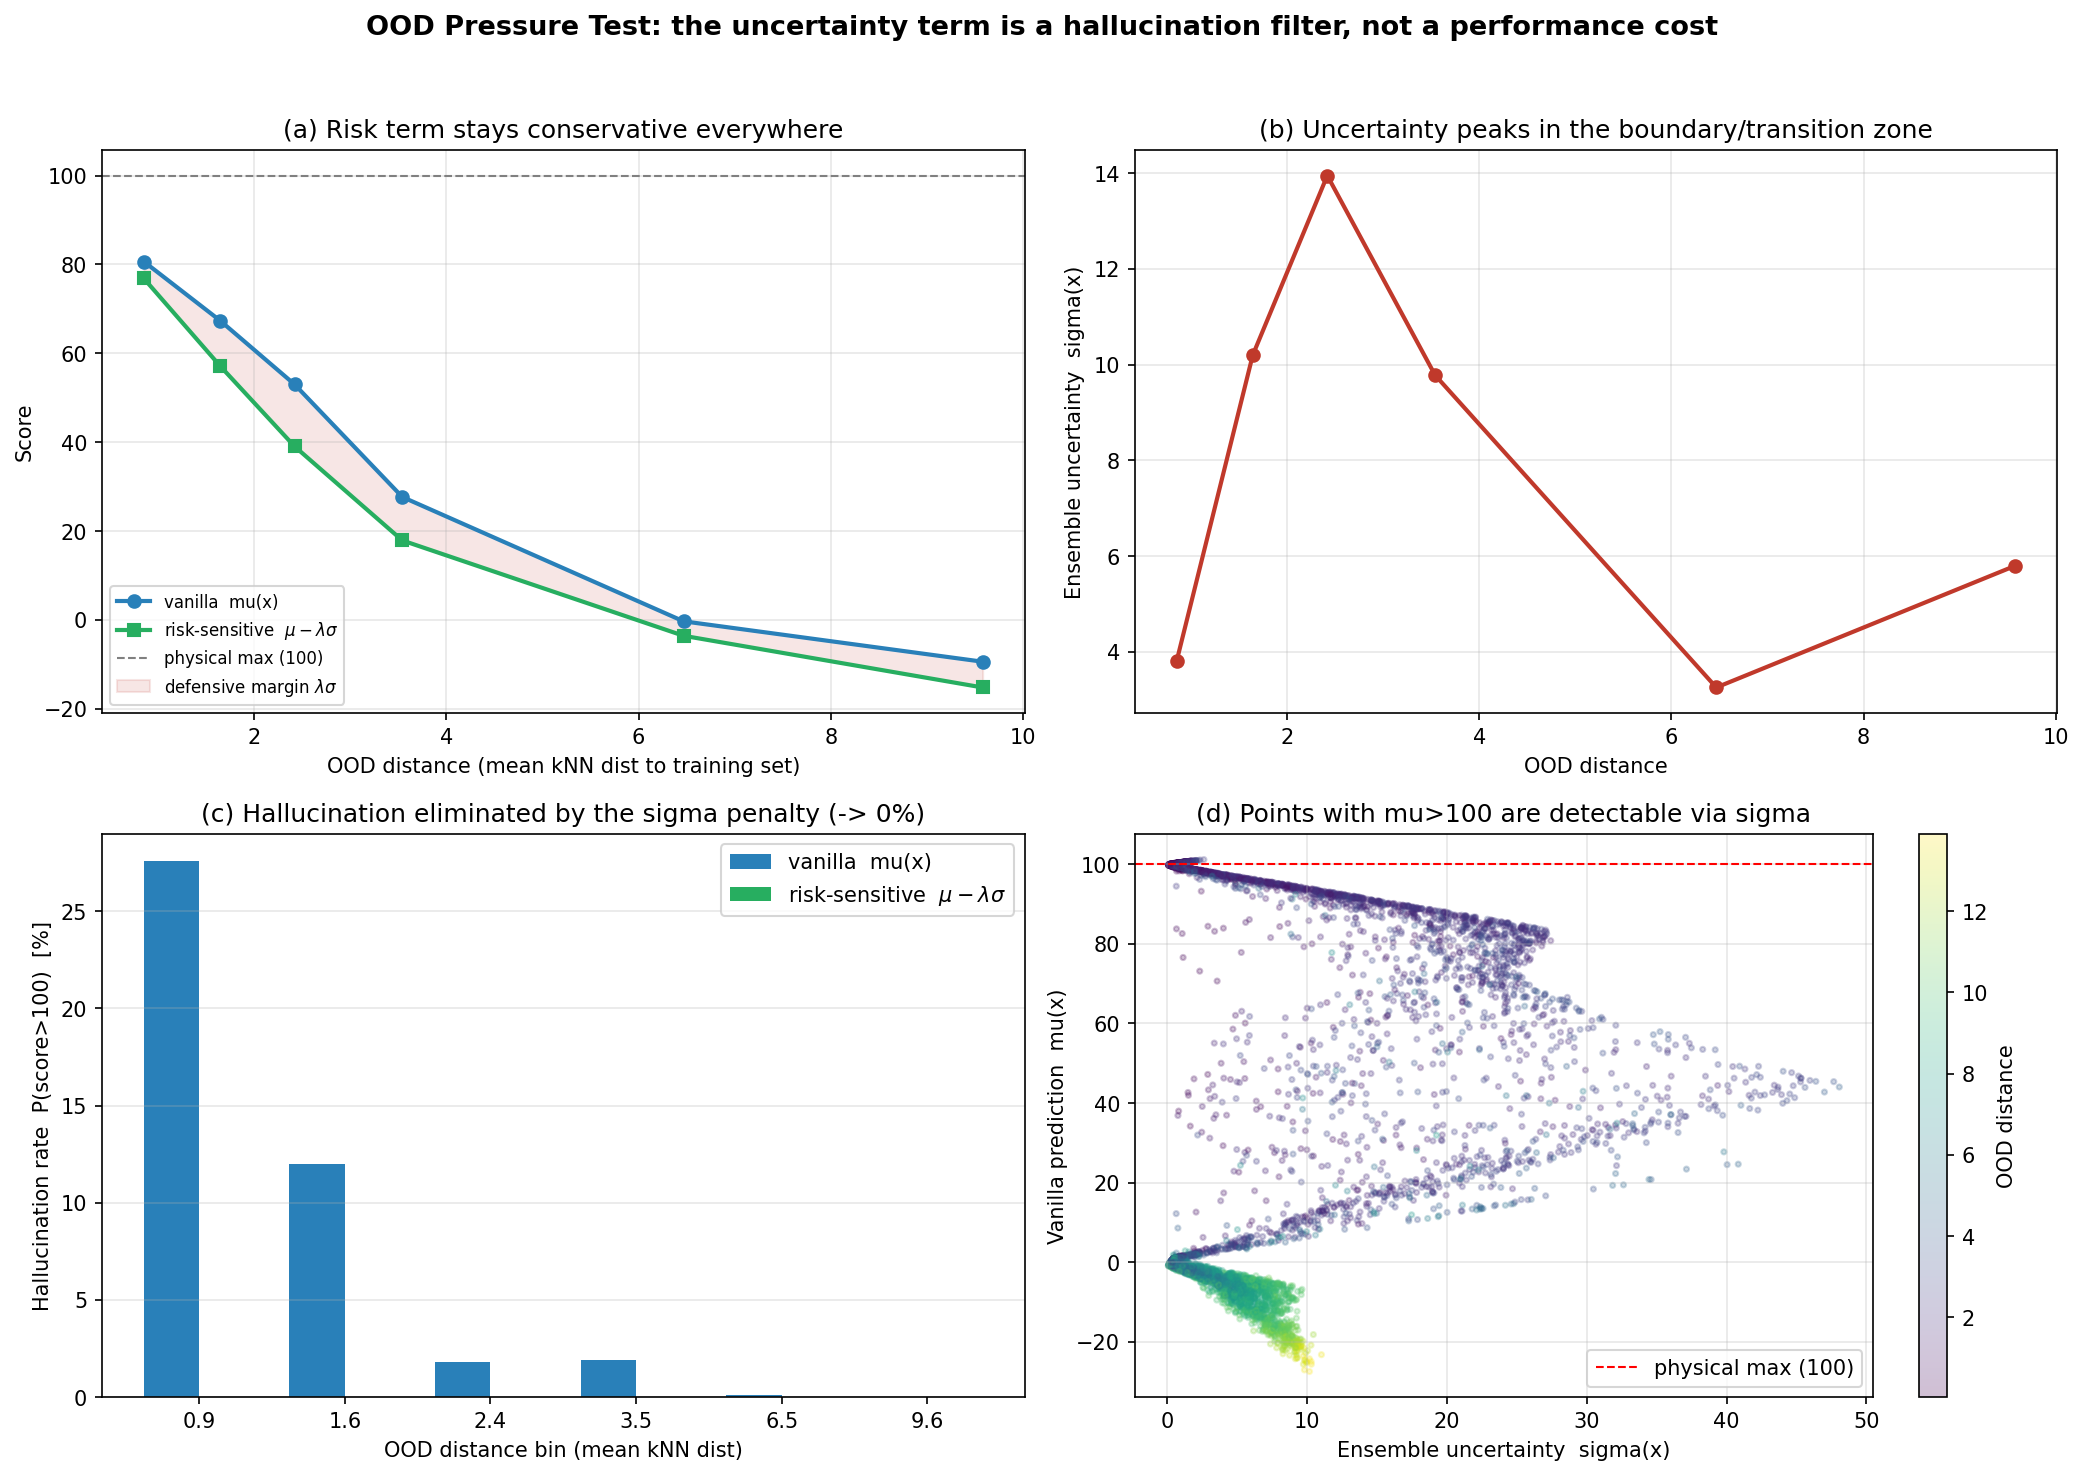
\includegraphics[width=0.95\textwidth]{figures/17_ood_stress.png}
\caption{风险敏感目标对分布外预测的抑制作用}
\label{fig:ood}
\end{figure}

图~\ref{fig:ood} 及统计结果表明：
\begin{enumerate}
    \item \textbf{原始代理存在过度外推}：vanilla $\mu(x)$ 最高达 \textbf{101.15}（$>100$）；
        在高稳定盆地边缘（最近邻区），约 \textbf{27.6\%} 的预测越过 100，
        而该区域正是仅追求高 $\mu$ 的优化器倾向访问的位置。
    \item \textbf{风险项抑制过度外推}：施加 $\lambda\sigma$ 后，
        $P(\mu-\lambda\sigma>100)$ 在所有密度区间均降为 \textbf{0\%}，
        最高风险敏感评分被约束在 $99.8$，回到物理合理区间。
    \item \textbf{不确定性可标识低可信区}：$\sigma(x)$ 在分布边界/过渡带达到峰值
        （均值 $13.95$，而盆地内仅 $3.81$、深 OOD 处 $5.80$），
        为优化器提供了该区域低可信的信号。
\end{enumerate}

这与消融实验（第~\ref{sec:converge}~节）一致：移除 $\sigma$ 惩罚（$\lambda=0$）后
适应度升至 \textbf{101.30}，过度外推重现。
因此 $\sigma$ 惩罚不应理解为性能损耗，而是面向 OOD 的防护：
其代价（$100.27\to99.83$，约 $0.4$ 分）换取的是将解约束在可信区间内。
密度惩罚 $D(x)$ 作为辅助引导项亦被实现，
但单独使用时因尺度设置过强而过度保守（适应度仅 $60.25$），
故在主流程中仅与 $\sigma$ 惩罚协同。

\subsection{盲区来源的进一步问题}

风险敏感优化约束了优化器对低可信区域的访问，
但仍遗留一个问题：为什么某些区域具有较高的不确定性？
一个合理的假设是训练数据在这些区域覆盖不足，代理因缺乏证据而预测不可靠。
若该假设成立，这些高 $\sigma$ 区域即为代理的认知盲区。
第~\ref{sec:refine}~节通过不确定性引导的数据精炼，检验这些盲区是否真实存在。
